\documentclass[12pt]{article}
\usepackage[margin=1in]{geometry}
\usepackage{setspace}
\onehalfspacing

% Start of preamble
%==========================================================================================%
% Required to support mathematical unicode
\usepackage[warnunknown, fasterrors, mathletters]{ucs}
\usepackage[utf8x]{inputenc}

\usepackage[dvipsnames,table,xcdraw]{xcolor}

% Standard mathematical typesetting packages
\usepackage{amsmath,amssymb,amscd,amsthm,amsxtra, pxfonts}
\usepackage{mathtools,mathrsfs,dsfont,xparse}

% Symbol and utility packages
\usepackage{cancel, textcomp}
\usepackage[mathscr]{euscript}
\usepackage[nointegrals]{wasysym}
\usepackage{apacite}

% Extras
\usepackage{physics}  
\usepackage{tikz-cd} 
\usepackage{microtype}
\usepackage{enumitem}
\usepackage{titling}
\usepackage{graphicx}

% Fancy theorems due to @intuitively on discord
\usepackage{mdframed}
\newmdtheoremenv[
backgroundcolor=NavyBlue!30,
linewidth=2pt,
linecolor=NavyBlue,
topline=false,
bottomline=false,
rightline=false,
innertopmargin=10pt,
innerbottommargin=10pt,
innerrightmargin=10pt,
innerleftmargin=10pt,
skipabove=\baselineskip,
skipbelow=\baselineskip
]{mytheorem}{Theorem}

\newenvironment{theorem}{\begin{mytheorem}}{\end{mytheorem}}

\newtheorem{corollary}{Corollary}
\newtheorem{lemma}{Lemma}

\newtheoremstyle{definitionstyle}
{\topsep}%
{\topsep}%
{}%
{}%
{\bfseries}%
{.}%
{.5em}%
{}%
\theoremstyle{definitionstyle}
\newmdtheoremenv[
backgroundcolor=Violet!30,
linewidth=2pt,
linecolor=Violet,
topline=false,
bottomline=false,
rightline=false,
innertopmargin=10pt,
innerbottommargin=10pt,
innerrightmargin=10pt,
innerleftmargin=10pt,
skipabove=\baselineskip,
skipbelow=\baselineskip,
]{mydef}{Definition}
\newenvironment{definition}{\begin{mydef}}{\end{mydef}}

\newtheorem*{remark}{Remark}

\newtheorem*{example}{Example}

% Common shortcuts
\def\mbb#1{\mathbb{#1}}
\def\mfk#1{\mathfrak{#1}}

\def\bN{\mbb{N}}
\def \C{\mbb{C}}
\def \R{\mbb{R}}
\def\bQ{\mbb{Q}}
\def\bZ{\mbb{Z}}
\def \cph{\varphi}
\renewcommand{\th}{\theta}
\def \ve{\varepsilon}
\newcommand{\mg}[1]{\| #1 \|}

% Often helpful macros
\newcommand{\floor}[1]{\left\lfloor#1\right\rfloor}
\newcommand{\ceil}[1]{\left\lceil#1\right\rceil}
\renewcommand{\qed}{\hfill\qedsymbol}
\renewcommand{\P}{\mathbb P\qty}
\newcommand{\E}{\mathbb{E}\qty}
\newcommand{\Cov}{\mathrm{Cov}\qty}
\newcommand{\Var}{\mathrm{Var}\qty}

% Sets
\usepackage{braket}

\graphicspath{{/}}
\usepackage{float}

\usepackage{booktabs}

\newcommand{\SET}[1]{\Set{\mskip-\medmuskip #1 \mskip-\medmuskip}}

% End of preamble
%==========================================================================================%

% Start of commands specific to this file
%==========================================================================================%

\renewcommand{\ip}[1]{\langle #1 \rangle}

%==========================================================================================%
% End of commands specific to this file

\title{CSE 422 Hw3}
\date{\today}
\author{Rohan Mukherjee}

\begin{document}
    \maketitle
    \textbf{Throughout this homework, whenever I report the usual training loss (non-normalized), I will always report the average training loss, instead of the sum.}
    \begin{enumerate}[leftmargin=\labelsep]
        \item \begin{enumerate}[label=(\alph*)]
            \item The value of the objective (average training loss) for $\hat \theta = (X^TX)^{-1} X^T y$ is 0.245766421039127 while for the all zeros vector it is 16.300105308625568.
            \item The test loss I got was 0.002693543440703437. This is indeed very small. It does not change very much for higher values of $m$, staying around the same thing. For extremely small values of $m$, like 1-10, there is a lot of variance, but it is still extremely small. This is probably because we sampled the data according to the rule $y = X \theta + \epsilon$ where $\epsilon$ is $N(0, 0.5I)$ random vector. Effectively, the data is just linear with some small noise. So the regression finds the parameter $\hat \theta$, which ends up being very close to the true parameter $\theta^*$. This is why the test loss is so small.
            \item I get the following table (with average training loss):
            \begin{table}
                \centering
                \caption{Model Performance Metrics}
                \label{tab:model_performance}
                \begin{tabular}{rrrr}
                \toprule
                   n &  Distance (theta\_hat - theta\_star) &  Training Loss &  Test Loss \\
                \midrule
                 500 &                             0.0944 &         0.2654 &     0.0094 \\
                1000 &                             0.0779 &         0.2511 &     0.0062 \\
                1500 &                             0.0517 &         0.2412 &     0.0027 \\
                2000 &                             0.0347 &         0.2422 &     0.0012 \\
                \bottomrule
                \end{tabular}
            \end{table}
            As you can see, the more training data we have, the lower the test loss (and usually the training loss) ends up being. This means that we are learning the parameter $\theta^*$ with more accuracy. Clearly, the test loss correlates more with the l2 distance than the training loss. I think this is because the training loss can only get so good, since there is noise in the loss function for the training data, but the test loss does not have any noise associated with it. Since we are learning $\theta^*$ with more accuracy the more training data we have, the test loss decreases accordingly with the l2 norm.

            \item For fixed $\theta$ and $\theta^*$, we know that, by i.i.d. of the training data,
            \begin{align*}
                \E(\frac 1m \sum (\ip{\theta^*, \hat x_i} - \ip{\theta, \hat x_i})^2) &= \frac 1m \sum \E((\ip{\theta^* - \theta, \hat x_i})^2) = \E(\ip{\theta^* - \theta, x_1}^2)\\
            \end{align*}
            Now recall that if $X = (X_1, \ldots, X_n)$ is a $N(0,I)$ random vector, then for $a \in R^n$, $\ip{a, X} = \sum a_iX_i$ is distributed according to $N(0, \mg{a}^2)$. Then the expression above is precisely the variance of the random variable $\ip{\theta^* - \theta, x_1}$, which by this short calculation is just $\mg{\theta - \theta^*}^2$. 

            \item By chain rule, $\nabla_\theta L_i(\theta) = \nabla_\theta (\theta^T x_i - y_i)^2 = 2(\theta^T x_i - y_i) \nabla_\theta [\theta^T x_i - y_i]$. Finally using that $\nabla_x a^Tx = a$, we get that this equals $2(\theta^T x_i - y_i) x_i$. Then the gradient of $L_{\text{train}}$ is just the sum of these gradients, which is $2 \sum x_i (x_i^T \theta - y_i)$. If $X$ is the matrix with $x_i^T$ as the $i$th row (and hence $x_i$ is a column vector), then this just equals $2X^T(X\theta - y)$. 

            For regular gradient descent, I get the following graph:
            \begin{figure}[H]
                \centering
                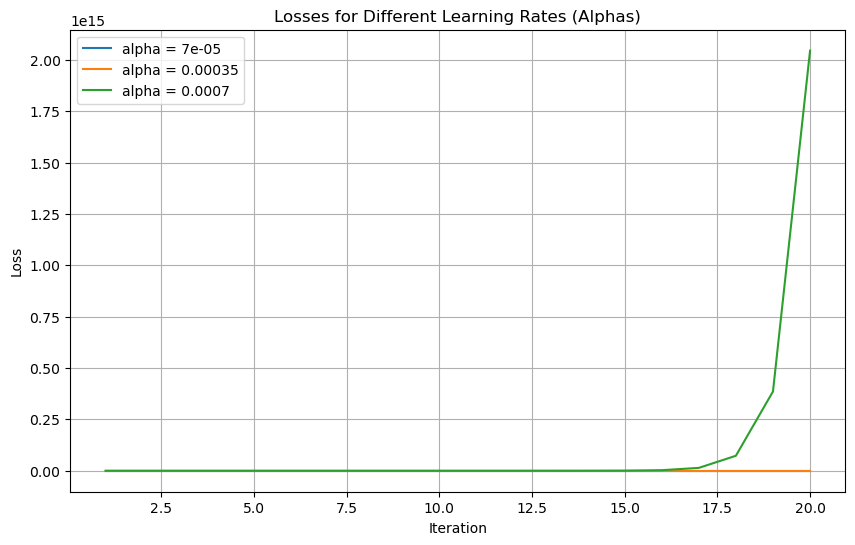
\includegraphics[width=0.8\textwidth]{grad_descent_output.png}
                \caption{Gradient Descent}
                \label{fig:gd}
            \end{figure}

            I get the following table for the final (average) training loss:
            \begin{table}[H]
                \centering
                \caption{Alpha vs Final Training Loss}
                \label{tab:alpha_vs_loss}
                \begin{tabular}{rr}
                \toprule
                  Alpha &  Final Training Loss \\
                \midrule
                0.00007 &         2.553572e-01 \\
                0.00035 &         2.553122e-01 \\
                0.00070 &         2.044280e+15 \\
                \bottomrule
                \end{tabular}
            \end{table}

            As you can see, the best training loss is achieved by the second one, $\alpha = 0.00035$. The first one is also really good. The last one is absolutely terrible. I think this is an example of it got to the min, as you can see in the graph, then overstepped the min and then the gradient started exploding, and it runs quickly away from the local minimum it had found. I also believe for learning rates that were too small, like something $1e-10 \ll 7e-5$ that worked well, it just would take too long to converge to the minimum. 0.00035 feels like a good middle ground.

            \item
            Pseudocode for SGD is as follows:
            \begin{enumerate}
                \item Initialize $\theta$ to 0
                \item For $t = 1, 2, \ldots, T$:
                \begin{enumerate}
                    \item Sample $i$ uniformly at random from $\{1, \ldots, n\}$
                    \item $\theta = \theta - \alpha \nabla L_i(\theta)$
                \end{enumerate}
                \item Return $\theta$
            \end{enumerate}

            \item The graph I get for SGD for $T = 20,000$ iterations is as follows:
            \begin{figure}[H]
                \centering
                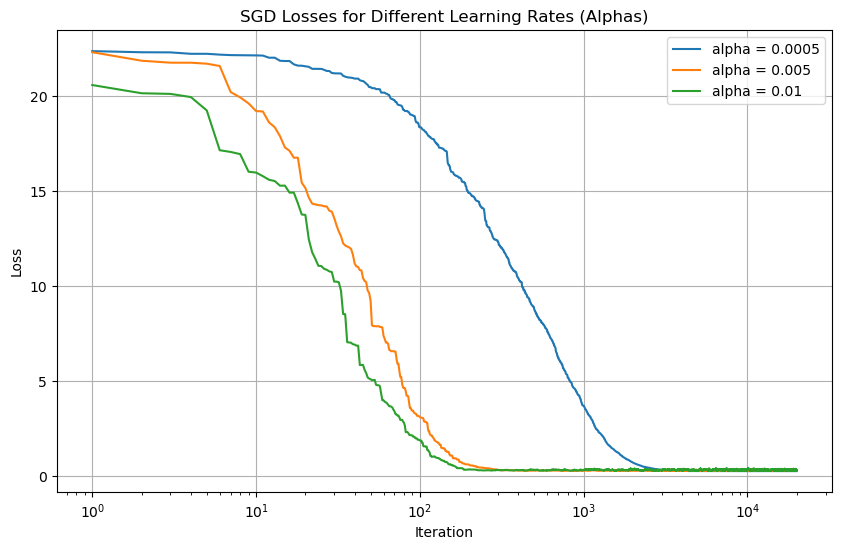
\includegraphics[width=0.8\textwidth]{sgd_output.png}
                \caption{SGD}
                \label{fig:sgd}
            \end{figure}
            The final objective values are like this:
            \begin{table}[H]
                \centering
                \caption{Final Objective Values for Different Alpha}
                \label{tab:final_objective_values}
                \begin{tabular}{rr}
                \toprule
                 Alpha &  Final Objective Value \\
                \midrule
                0.0005 &               0.254497 \\
                0.005 &               0.262516 \\
                0.01 &               0.338374 \\
                \bottomrule
                \end{tabular}
            \end{table}
            Pictorially, they all look around the same, and the final output values reflects that. However, as expected, the larger the $\alpha$ the larger the final objective value. This is because the larger $\alpha$ introduces more variance into the SGD process, leading to the very small fluctuations in the objective value you can see in the image. From a previous part, $\nabla_\theta L_i(\theta) = 2(\theta^T x_i - y_i)x_i$. So, the function uses precisely one data point per iteration. Since we run for $T = 10,000$ iterations, and there are 2,000 training samples, we use each smaple 5 times on average. This is much better than the 20 times we used them in the gradient descent part. It also gets the same final output value, which is interesting.

            \item 
            My intuition is that if the gradient is large, this means that the minimum is very far away. So we should probably move even more than the small learning rate we have put. On the other hand, if the gradient is small, and we had the same constant learning rate, we would overstep the minimum, and the loss would increase. So I propose that we use a step size proportional to the size of $\nabla L_i(\theta)$, such as its absolute max coordinate (I would suspect that this is faster to compute than the norm of the gradient).

            I have tried the following, where $\alpha_0$ is a hyperparameter and $d$ is the length of the input samples:
            \begin{enumerate}
                \item $\alpha_t = \frac{\alpha_0}{d} \max_{j} |\nabla L_i(\theta)|$
                \item $\alpha_t = \frac{\alpha_0}{d} \|\nabla L_i(\theta)\|$
                \item $\alpha_t = \frac{\alpha_0}{t}$
            \end{enumerate}
            Here are the plots, in order:
            \begin{figure}[H]
                \centering
                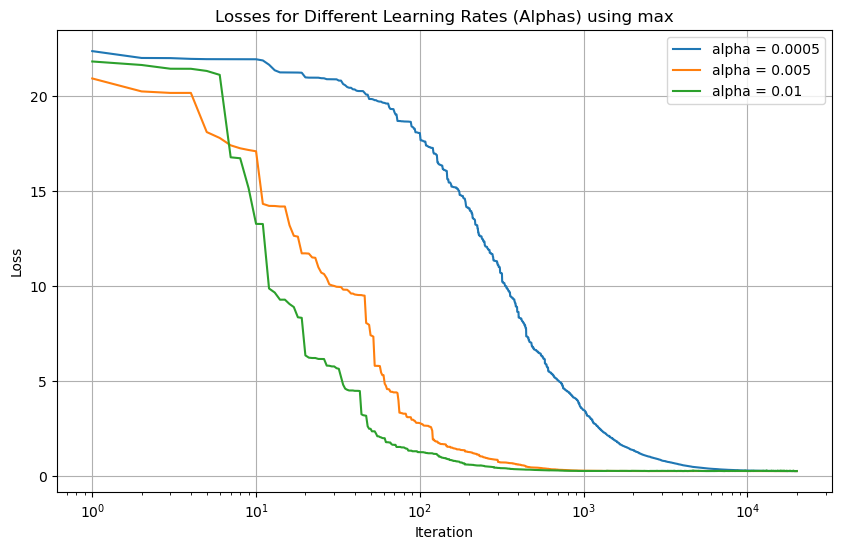
\includegraphics[width=0.8\textwidth]{sgd_max.png}
                \caption{$\alpha_t = \frac{\alpha_0}{d} \max_{j} |\nabla L_i(\theta)|$}
                \label{fig:adaptive_alpha_1}
            \end{figure}
            \begin{figure}[H]
                \centering
                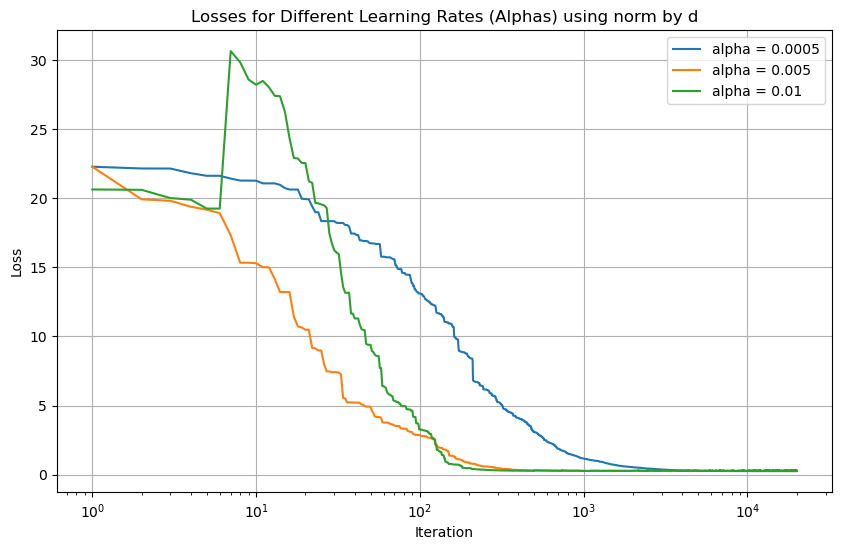
\includegraphics[width=0.8\textwidth]{sgd_norm_d.png}
                \caption{$\alpha = \frac{\alpha_0}{d} \|\nabla L_i(\theta)\|$}
                \label{fig:adaptive_alpha_2}
            \end{figure}
            \begin{figure}[H]
                \centering
                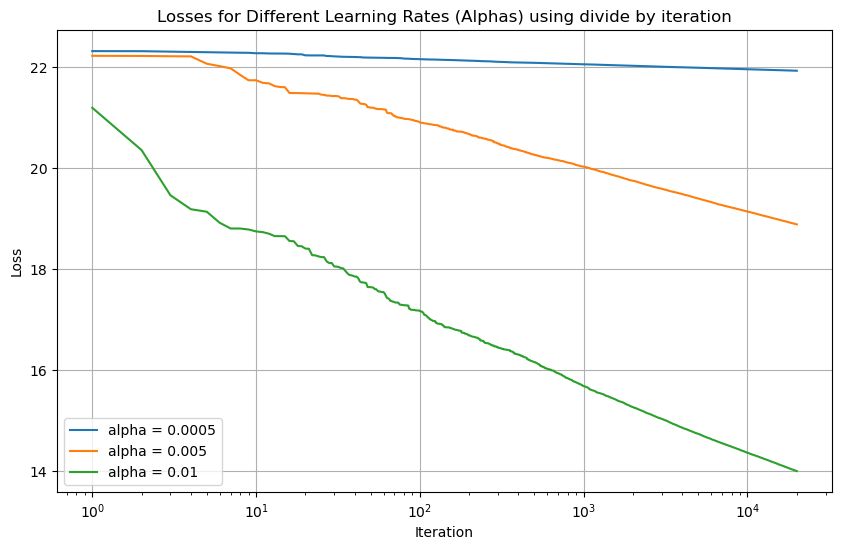
\includegraphics[width=0.8\textwidth]{sgd_it.png}
                \caption{$\alpha_t = \frac{\alpha_0}{t}$}
                \label{fig:adaptive_alpha_3}
            \end{figure}
            The tables are:
            \begin{table}[H]
                \centering
                \begin{tabular}{c c}
                    \toprule
                    $\alpha$ & Final Loss \\
                    \midrule
                    0.0005 & 0.2554149788012268 \\
                    0.005  & 0.25913216028792124 \\
                    0.01   & 0.27304750826263313 \\
                    \bottomrule
                \end{tabular}
                \caption{Final loss values using max.}
            \end{table}
            
            \begin{table}[H]
                \centering
                \begin{tabular}{c c}
                    \toprule
                    $\alpha$ & Final Loss \\
                    \midrule
                    0.0005 & 0.2547512193059818 \\
                    0.005  & 0.26364601860013565 \\
                    0.01   & 0.28366985519259025 \\
                    \bottomrule
                \end{tabular}
                \caption{Final loss values using norm / d.}
            \end{table}
            
            \begin{table}[H]
                \centering
                \begin{tabular}{c c}
                    \toprule
                    $\alpha$ & Final Loss \\
                    \midrule
                    0.0005 & 22.04319880187047 \\
                    0.005  & 17.55662684111231 \\
                    0.01   & 15.383248856596401 \\
                    \bottomrule
                \end{tabular}
                \caption{Final loss values using divide by iteration.}
            \end{table}
            The best one is the first option I used as you can see, which is $\alpha_t = t \frac{\alpha_0}{d} \max_{j} |\nabla L_i(\theta)|$. The last one is really bad as it does not follow the general pipeline I first proposed and instead i just proportional to the iteration, but this doesn't look at all to see how close we are to a local min like the other two methods try to do. I suspect that the first method, using only the max coordinate instead of the full norm of the gradient, has smaller variance since it uses a smaller value. As you can also see for the max alpha, it seems to converge at around the same rate as the first one, being almost done at iteration 100, but it is much more stable, as the 0.01 learning rate has a lot less variance then in the normal SGD.
        \end{enumerate}

        \item \begin{enumerate}
            \item We were told to ignore the written part for this question in an email.
            I get, over 10 trials, an average train loss of 1.1304786543239968e-11 and an average test loss of 1.2260962605261125. We can see an insane amount of overfitting here.

            \item Here is the plot of the choice of $\lambda$ vs training and test loss:
            \begin{figure}[H]
                \centering
                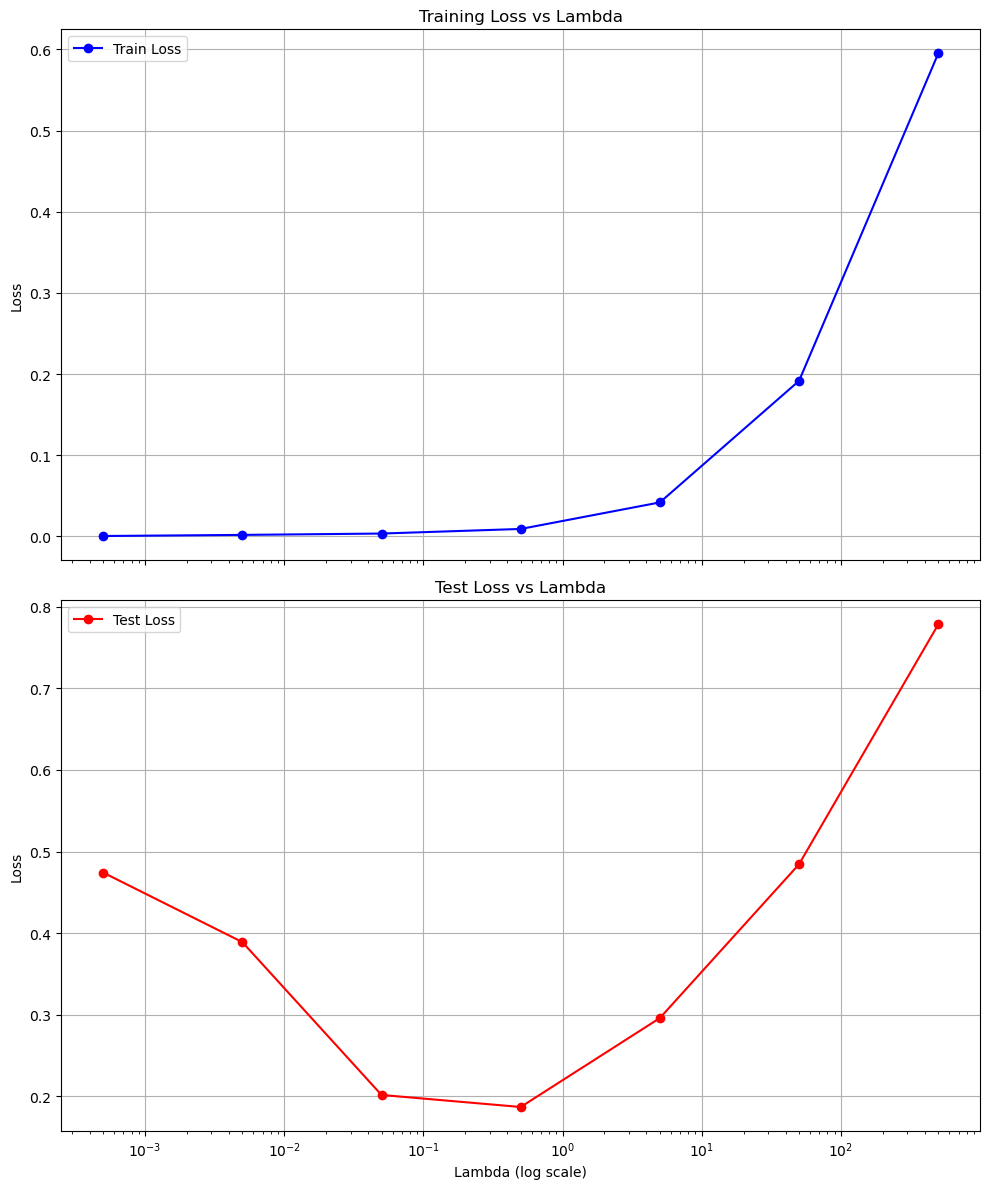
\includegraphics[width=0.8\textwidth]{loss_vs_lambda.png}
                \caption{Ridge Regression}
                \label{fig:ridge}
            \end{figure}
            We can see a lot of overfitting for the smaller lambdas, like $\lambda < 10^{-1}$. In the picture, the training loss keeps going down but the test loss starts going up. However, compared to part (a) where the test loss was like 11 orders of magnitude smaller than the training loss, this is much better! We don't get anywhere near that kind of overfitting, which is great. It seems like the best $\lambda$ is slightly lower than 1.

            \item Running SGD on the orginal loss function yields:
            \begin{table}[H]
                \centering
                \begin{tabular}{|c|c|c|}
                    \hline
                    \textbf{Alpha} & \textbf{Average Train Loss} & \textbf{Average Test Loss} \\
                    \hline
                    $5 \times 10^{-5}$ & 0.0119 & 0.2009 \\
                    \hline
                    $5 \times 10^{-4}$ & 0.0047 & 0.1816 \\
                    \hline
                    $5 \times 10^{-3}$ & $\infty$ & $\infty$ \\
                    \hline
                \end{tabular}
                \caption{Effect of Different Learning Rates on Training and Testing Loss}
                \label{tab:learning_rates}
            \end{table}
            This solution absolutely blows the first one out of the water. Without even doing any explicit regularization, it beats the best ridge solution. Wow. 

            \item Here is the plot of the train loss vs converging $\alpha$, test loss vs converging $\alpha$ and l2 norm vs converging $\alpha$:
            \begin{figure}[H]
                \centering
                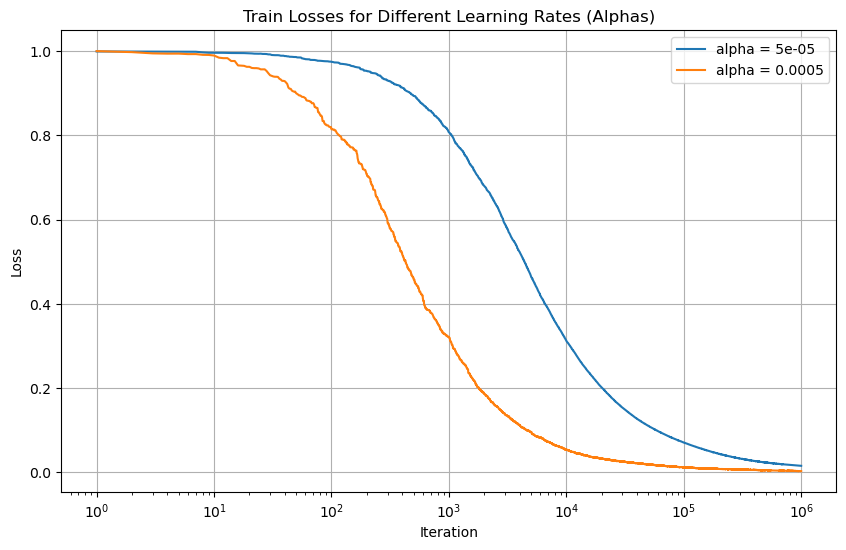
\includegraphics[width=0.8\textwidth]{train_wrt_alpha.png}
                \caption{Converging Alpha}
                \label{fig:converging_alpha}
            \end{figure}

            \begin{figure}[H]
                \centering
                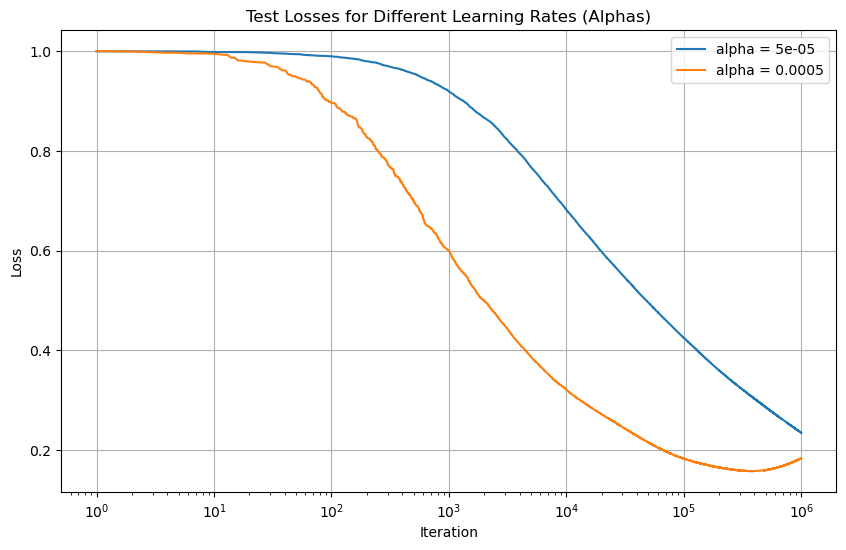
\includegraphics[width=0.8\textwidth]{test_wrt_alpha.png}
                \caption{Converging Alpha}
                \label{fig:converging_alpha}
            \end{figure}

            \begin{figure}[H]
                \centering
                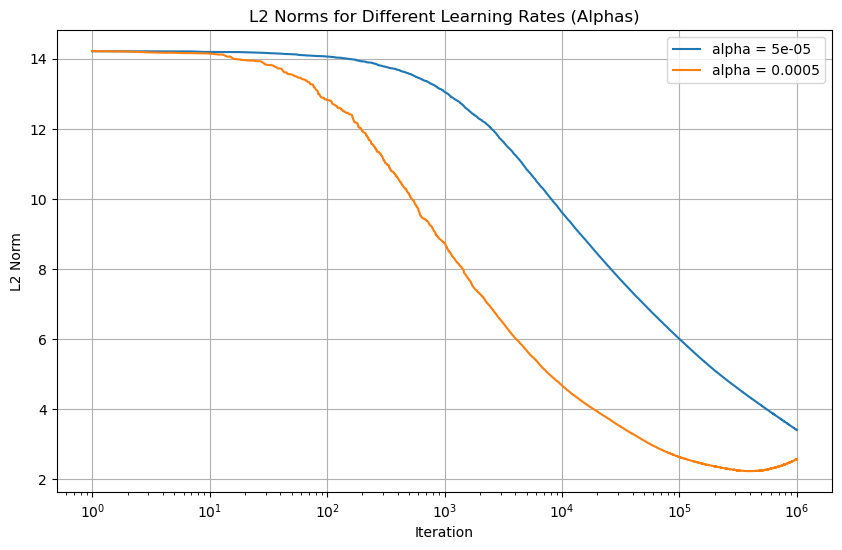
\includegraphics[width=0.8\textwidth]{l2_wrt_alpha.png}
                \caption{Converging Alpha}
                \label{fig:converging_alpha}
            \end{figure}
            SGD seems to generalize extremely well with different step sizes. Although they converge at different rates, as you can see, since it doesn't seem to overfit until maybe at the very end, and seems to be constantly converging towards a minimum. It seems that the amount that a specific $\alpha$ generalizes is positively correlated with the $\ell^2$ norm of the distance between $\hat \theta$ and $\theta^*$, which makes sense. If we had a perfect $\hat \theta = \theta^*$ then the test loss would be 0. So test loss is very related to the distance.
        \end{enumerate}

        \item When we have $d = 300$ dimensions and $n = 200$ training points, we saw above that equal amounts of training data and dimensions works really well with SGD, and the full gradient optimizaiton problem does not. So I will use a form of SGD, as it seems from above to generalize better. I also don't want to have to worry about learning rates, so I will use the adaptive learning rate that I found above works well, $\alpha_t = \frac{\alpha_0}{d} \max_{j} |\nabla L_i(\theta)|$. I ran a hyperparameter search over $\alpha \in \SET{0.00005, 0.0005, 0.005}$ and $\lambda \in \SET{0.0005, 0.005, 0.05, 0.5, 5}$. I learned that $T = 10,000$ iterations wasn't enough to converge, so I ended up using $T = 100,000$ iterations. After searching through the entire $(\alpha, \lambda)$ hyperparameter space, the best parameters I got were $\alpha = 0.0005$ and $\lambda = 0.05$ with final average normalized train loss of 0.07226665890624548 and the best normalized test loss I got was 0.592696195064302. This wasn't very good but the data is very noisy and we don't have a lot of data, so in the grand scheme of things it is probably okay.
    \end{enumerate}
\end{document}